\documentclass[10pt]{article}

\usepackage{fullpage}
\usepackage{graphicx}
\usepackage[ngerman]{babel}
\usepackage[utf8]{inputenc}

\title{Dokumentation des Go-Projekts}
\author{Von 2416160, 5836402}
\date{}

\begin{document}
    \maketitle
	\section{Architekturdokumentation}
    \begin{figure}[h]
        \centering
        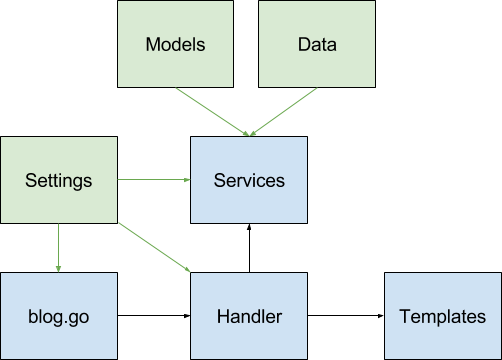
\includegraphics[width=0.8\textwidth]{Architektur.png}
        %		\vspace{5mm}
        \caption{Zusammenhang der einzelnen Komponenten}
        \label{img:architektur}
    \end{figure}
    In Abbildung \ref{img:architektur} ist eine Übersicht über die Komponenten zu sehen. Die blauen Komponenten sind
    Teil des Funktionsflusses und die grünen stellen Datenelemente dar. Das Programm beginnt in der Routine
    \textit{blog.go} und registriert dort alle Handler. Außerdem ist dort das REPL umgesetzt. Bei Aufruf einer gültigen
    URL wird der entsprechende Handler aufgerufen. Ein Handler ruft je nach Bedarf ein oder mehrere Services auf um
    Daten abzurufen oder Funktionen auszuführen. Zum Beispiel kann er vom \textit{sessionService} die aktuelle Session
    abfragen oder eine neue erstellen lassen sofern noch keine vorhanden ist. Die Session wird ihm dann in Form eines
    \textit{structs}, das in Models definiert ist, übergeben. Alle verwendeten \textit{structs} sind im Package ''models''
    definiert. Im Package ''data'' liegen alle Daten-Dateien für die Settings, die BlogPosts und die User, also alle Daten
    die persistent gespeichert werden sollen. Die Settings sind hier nochmals besonders hervorgehoben, da sie zur
    Laufzeit im Speicher global allen Funktionen zur Verfügung stehen sollen. Aus diesem Grund liegt ihre Instanz im
    Package ''global''. Hat ein Handler alle Daten die er braucht und alle nötigen Funktionen ausgeführt, so wird er
    entweder ein Template rendern und diesem Daten mitgeben oder einen Redirect auf einen anderen Handler starten.

	\section{Anwenderdokumentation}
	Beim Aufruf der Seite (lokal via "localhost") wird der Nutzer direkt auf die gesicherte https-Ansicht umgeleitet.
	Auf der Startseite wird dem Nutzer der aktuellste Post dargestellt, falls verf\"ugbar.
	Unter der \"Uberschrift befindet sich ein Link zur Archivdarstellung, auf der sich alle Posts befinden, der sich auf der Archivdarstellung zu einem Link auf die Startseite \"andert.
	Alle Posts sind mit den zugeh\"origen Kommentaren unterlegt, die von jedem Nutzer erstellt werden k\"onnen.
	Vorausgesetzt der Nutzer besitzt ein Authorenkonto, kann er sich am unteren Ende der Seiten \"uber den Link "Login" einloggen.
	Auf der Seite befinden sich lediglich die Felder f\"ur den Benutzernamen und das Passwort, bei Fehlschl\"agen wird ein Fehler angezeigt (z.B. "Falsches Passwort").
	
	Ist der Nutzer erfolgreich eingeloggt, kann er sich jederzeit \"uber den Link, wieder am unteren Ende der Seiten, ausloggen.
	Ebenfalls ist es eingeloggten Nutzern m\"oglich Posts zu verfassen, und zwar \"uber das Feld und den Button "New Post", jeweils am unteren Ende der Auflistungen der Posts auf der Index- und Archivseiten.
	Neben dem Logout Button am unteren Ende der Seite kann der eingeloggte Nutzer sein Passwort \"andern.
	Zuletzt ist es eingeloggten Nutzern m\"oglich ihre eigenen Posts aufzulisten, \"uber den Link "My Posts" am unteren Ende der Seite.
	Auf dieser Seite kann jeder Post einzeln editiert oder gel\"oscht werden.
	
	Nicht eingeloggte Nutzer die auf Authorenfunktionen zugreifen werden auf die Startseite zur\"ucknavigiert.
	\section{Inbetriebnahme}
		Der Server kann g\"anzlich ohne Anpassungen gestartet werden.
		Die Standardeinstellungen sehen wie folgt aus:
		\begin{tabular}{l|l}
			PortNumber &     4443\\
			SessionTimeout & 15\\
			PostSuffix & .json\\
			KeyFile & key.pem\\
			CertFile & cert.pem\\
		\end{tabular}\\
		Die Standardeinstellungen werden von den Einstallungen in der settings-Datei \"uberschrieben, die wiederum von den Einstellungen der CommandLine Parameter \"uberschreibene werden, vorrausgesetzt diese existieren jeweils.

		Standardm\"a{\ss}ig ist auch ein root Benutzer eingerichtet, der folgende Logindaten hat: Name: "root", Passwort:"toor".
		\subsection{Serverinformationen via REPL}
		\"Uber einen sog. "Read Eval Print Loop" ist es m\"oglich im laufenden Betrieb Informationen abzurufen.
		Das Kommando "?" zeigt die Befehle an, die akzeptiert werden. Die Befehle sehen folgenderma{\ss}en aus:\\\\
		\begin{tabular}{l|l|l}
			Kommando   & Effekt   & Beschreibung\\
			\hline
			q          & quit     & Beendet den Server\\
			s          & settings & Gibt die aktuell aktiven Einstellungen aus\\
			v          & version  & Gibt die Versionsnummer aus\\
			u          & users    & Gibt alle aktiven User aus (alle Users mit Session)\\
			(r config) & -        & Undocumented: L\"adt die Konfiguration neu
		\end{tabular}
	\section{Beitrag zum Projekt}
		\subsection{2416160}
		\begin{itemize}
			\item Entwurf und Umsetzung der Templates (index, archive, login, changePassword, myPosts)
			\item Entwurf und Implementierung der BlogPost Funktionen (LoadPosts, GetPosts, Save-, New-, Change-, DeletePost)
			\item Entwurf und Implementierung der Settings Funktionen (Defaults, File und CommandLine Parameter)
			\item Entwurf und Umsetzung der Benutzerverwaltung
			\item Entwurf und Einbau der Krypto-Funktionen
			\item Entwurf und Bau des REPL's
			\item Einbau der Cookie Verwaltung
			\item Handler und Redirect (redirect to index, tls redirect) Logik
			\item Zertifikate
			\item Unit Tests f\"ur PostsService und UserService
			\item Dokumentation
		\end{itemize}
		\subsection{5836402}
\end{document}